\documentclass[12pt, oneside]{article}
\usepackage[letterpaper, margin=1in]{geometry}
\usepackage[english]{babel}
\usepackage[utf8]{inputenc}
\usepackage{amsmath}
\usepackage{amsfonts}
\usepackage{amssymb}
\usepackage{tikz}
\usepackage{tkz-fct}

\usepackage{fancyhdr}
\pagestyle{fancy}
\fancyhf{}
\rhead{\thepage \\Name: \hspace{1.5in}.\\}
\lhead{BECA / Dr. Huson / 11.2 Algebra 2 Regents prep \\* 22 May 2018 \\* \textbf{Homework: Polynomial functions and graphs}}

\vspace{1cm}

\renewcommand{\headrulewidth}{0pt}

\title{Problem set template}
\author{Chris Huson}
\date{May 2018}

\begin{document}
%\maketitle

\subsubsection*{\\* \textnormal{Graph carefully using pencil}}

\begin{enumerate}

\item A business has modeled it revenues and costs as functions of sales.\\[5pt] Revenues, $r$, in millions of dollars, are modeled as $r\left(x\right)=-0.15x^2+25x$, where $x$ is the sales in thousands.\\[5pt]
The function for costs, $c$, in millions of dollars, is $c\left(x\right)=0.015x^3-.5x^2+10x+120$\\*[5pt]
Graph each function on the set of axes below.
\begin{center}
    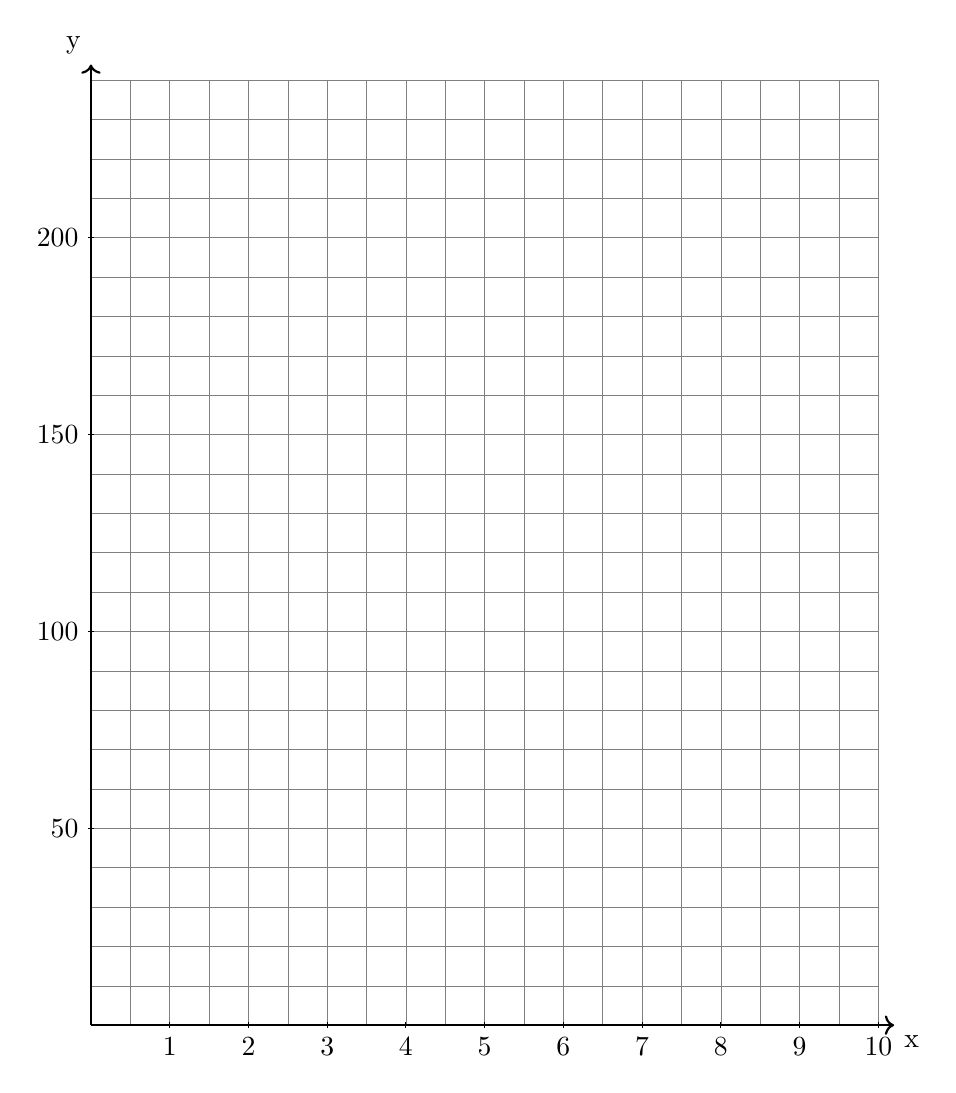
\begin{tikzpicture}[scale=4/4]
    \draw[step=0.5cm,gray,very thin] (0,0) grid (10,12);
    \draw[thick,->] (0,0) -- (10.2,0) node[anchor=north west] {x};
    \draw[thick,->] (0,0) -- (0,12.2) node[anchor=south east] {y};
    \foreach \x in {1,2,3,4,5,6,7,8,9,10} \draw (\x cm,1pt) -- (\x cm,-1pt) node[anchor=north] {$\x$};
    \foreach \y in {2.5} \draw (1pt,\y cm) -- (-1pt,\y cm) node[anchor=east] {50};
    \foreach \y in {5} \draw (1pt,\y cm) -- (-1pt,\y cm) node[anchor=east] {100};
    \foreach \y in {7.5} \draw (1pt,\y cm) -- (-1pt,\y cm) node[anchor=east] {150};
    \foreach \y in {10} \draw (1pt,\y cm) -- (-1pt,\y cm) node[anchor=east] {200};
    \end{tikzpicture}
\end{center}
What will the revenues be when the sales are 5 thousand? Round to the \emph{nearest million dollars}\\*[0.5in]
When will the company break even, in other words, for what $x$ will revenues and costs be equal, \emph{to nearest tenth}? 

\newpage

\item Sketch a graph with the following characteristics: 
\begin{itemize}
\item one positive, real zero
\item of degree two
\item positive leading coefficient
\end{itemize}
\begin{center}
    \begin{tikzpicture}[scale=2/4]
    \draw[thick,<->] (-7.5,0) -- (7.5,0) node[anchor=north west] {\textbf{x}};
    \draw[thick,<->] (0,-7.5) -- (0,7.5) node[anchor=south east] {\textbf{y}};
    \end{tikzpicture}
\end{center}


\item Sketch a graph with the following characteristics: 
\begin{itemize}
\item a cubic polynomial function
\item a negative leading coefficient
\item three real zeros, all negative
\end{itemize}
\begin{center}
    \begin{tikzpicture}[scale=2/4]
    \draw[thick,<->] (-7.5,0) -- (7.5,0) node[anchor=north west] {\textbf{x}};
    \draw[thick,<->] (0,-7.5) -- (0,7.5) node[anchor=south east] {\textbf{y}};
    \end{tikzpicture}
\end{center}



\end{enumerate}
\end{document}